
\section{Il contenuto e la navigabilità}

	\subsection{Il testo}
		Data la tipologia personale del sito internet non è richiesto che il testo abbia tante accortezze linguistiche come, per esempio, un sito giornalistico. Si è quindi analizzato che il testo rispettasse le regole base di usabilità:
		\begin{itemize}
			\item \textbf{Dimensione} del testo adatta e \textbf{leggibilità};
			\item Supporto dell'opzione \textbf{zoom} del browser;
			\item Tipologia di \textbf{font};
			\item \textbf{Contrasto} tra testo e sfondo;
			\item Presenza di una \textbf{Struttura} del testo;
		\end{itemize}
		
		\subsubsection{Dimensione e leggibilità}
			La dimensione del testo è impostata su 1em il che corrisponde a circa 12pt e quindi supera quella minima consigliata (10pt). Ogni parte del testo risulta sempre leggibile anche se l'utilizzo di testo in formato italico e in grassetto abbonda. Viene utilizzata spesso la scrittura in stampatello maiuscolo e questo se pur poco diminuisce l'usabilità dell'utenza abituata a leggere in stampatello minuscolo.
			
		\subsubsection{Zoom}
			Il sito non presenta un'opzione di zoom interna. Si è quindi provato ad utilizzare lo zoom implementato nel browser per analizzare se questo fosse supportato, ossia se la pagina degradasse elegantemente e mantenesse la leggibilità del testo. 
			La funzionalità zoom è permessa e nei maggiori browser (IE, Chrome, Firefox) funziona perfettamente, la leggibilità permane grazie al layout del sito responsive.
			L'uso invece della funzionalità di aumento della dimensione dei caratteri interna al browser invece non in tutto il testo viene applicata (i titoli rimangono quasi invariati), l'uso eccessivo però porta alla presenza della barra di scroll orizzontale. Non sarà considerato un punto negativo poiché penso che l'incremento della dimensione dei font nel browser non raggiunga mai quelle dimensioni.
	
		\subsubsection{Font}
			La tipologia del font è personalizzata, non presenta grazie ed è gradevole alla vista.
			
		\subsubsection{Contrasto}
			Molto spesso lo sfondo del testo è di colore bianco, per cui perfettamente leggibile anche se il colore non sempre è nero. Il testo sovrapposto alle immagini risulta sempre visibile grazie all'utilizzo di una sfumatura situata tra immagine e testo che mantiene il corretto contrasto.
			
		\subsubsection{Struttura}
			Il testo è sempre suddiviso in paragrafi con sottotitoli a sua volta suddivisi in blocchi di testo e durante l'analisi non si sono mai trovati muri di testo. Questo garantisce maggior leggibilità e incoraggia l'utente alla lettura. Alcune volte il testo risulta interrotto da immagini che possono interrompere la lettura dell'utente provocando frustrazione (figura \ref{fig:ImageBetweenText}). In tal caso un rimedio potrebbe essere di ridurre la dimensione delle immagini, affiancarle al testo e permettere che il click su di esse mostri lo zoom (attualmente questa possibilità esiste anche se il caricamento risulta eccessivamente lungo).
			
			\begin{figure} [h]
				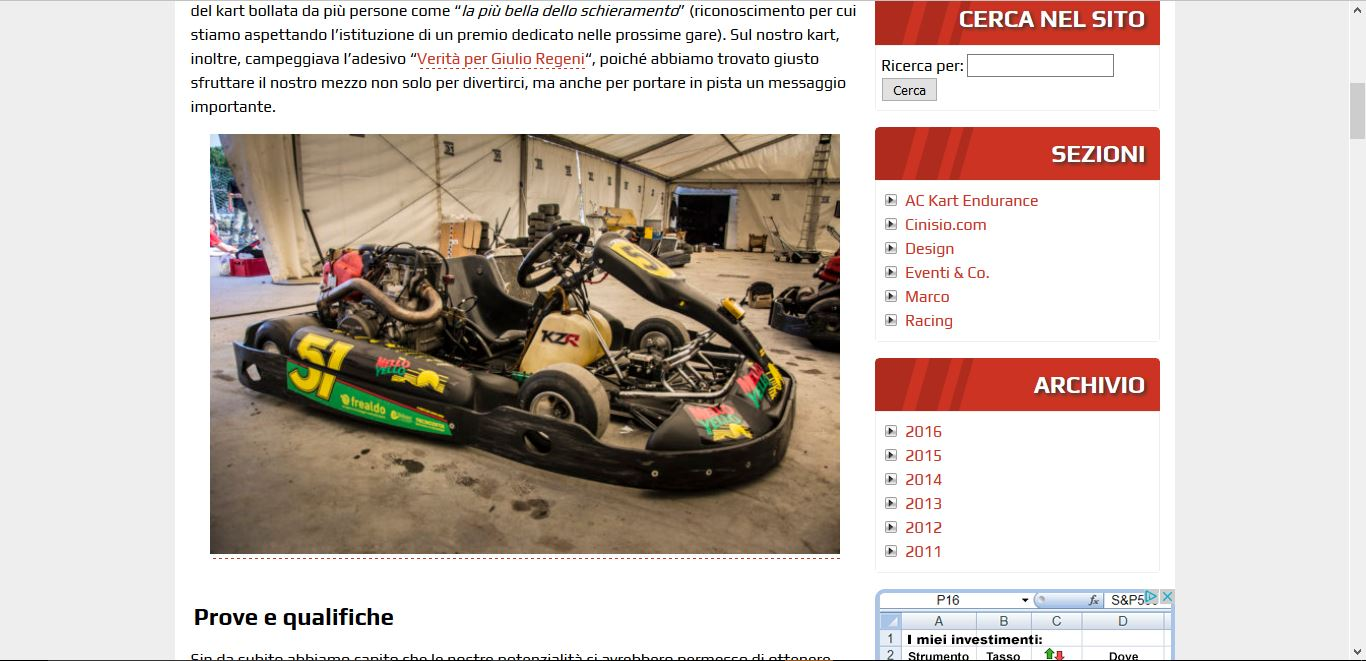
\includegraphics[width=\textwidth]{images/ImageBetweenText}
				\caption{Esempio di immagine che interrompe la lettura dell'articolo}
				\label{fig:ImageBetweenText}
			\end{figure}
			
	
	\newpage
	\subsection{Le immagini}
		Il sito presenta una grossa attenzione alle immagini alle quali sembra sia data più priorità rispetto al testo. Il numero di immagini in ogni pagina risulta molto elevato e spesso di troppo. Questo oltre ad occupare notevole spazio nella pagine con contenuto di poco interesse per l'utente medio comporta frustrazione, lo scanning iniziale della pagina(per esempio l'homepage), dato l'elevato numero di immagini, sarà quasi completamente bianco provocando disorientamento nell'utenza.
		
		A tal proposito si mostra nella figura \ref{fig:BlankHomepage1} la homepage completamente spoglia delle immagini, sicuramente il design si affievolisce ma questo si può considerare come quello che un utente visualizza nella fase dello scanning.
		
		\begin{figure} [h]
			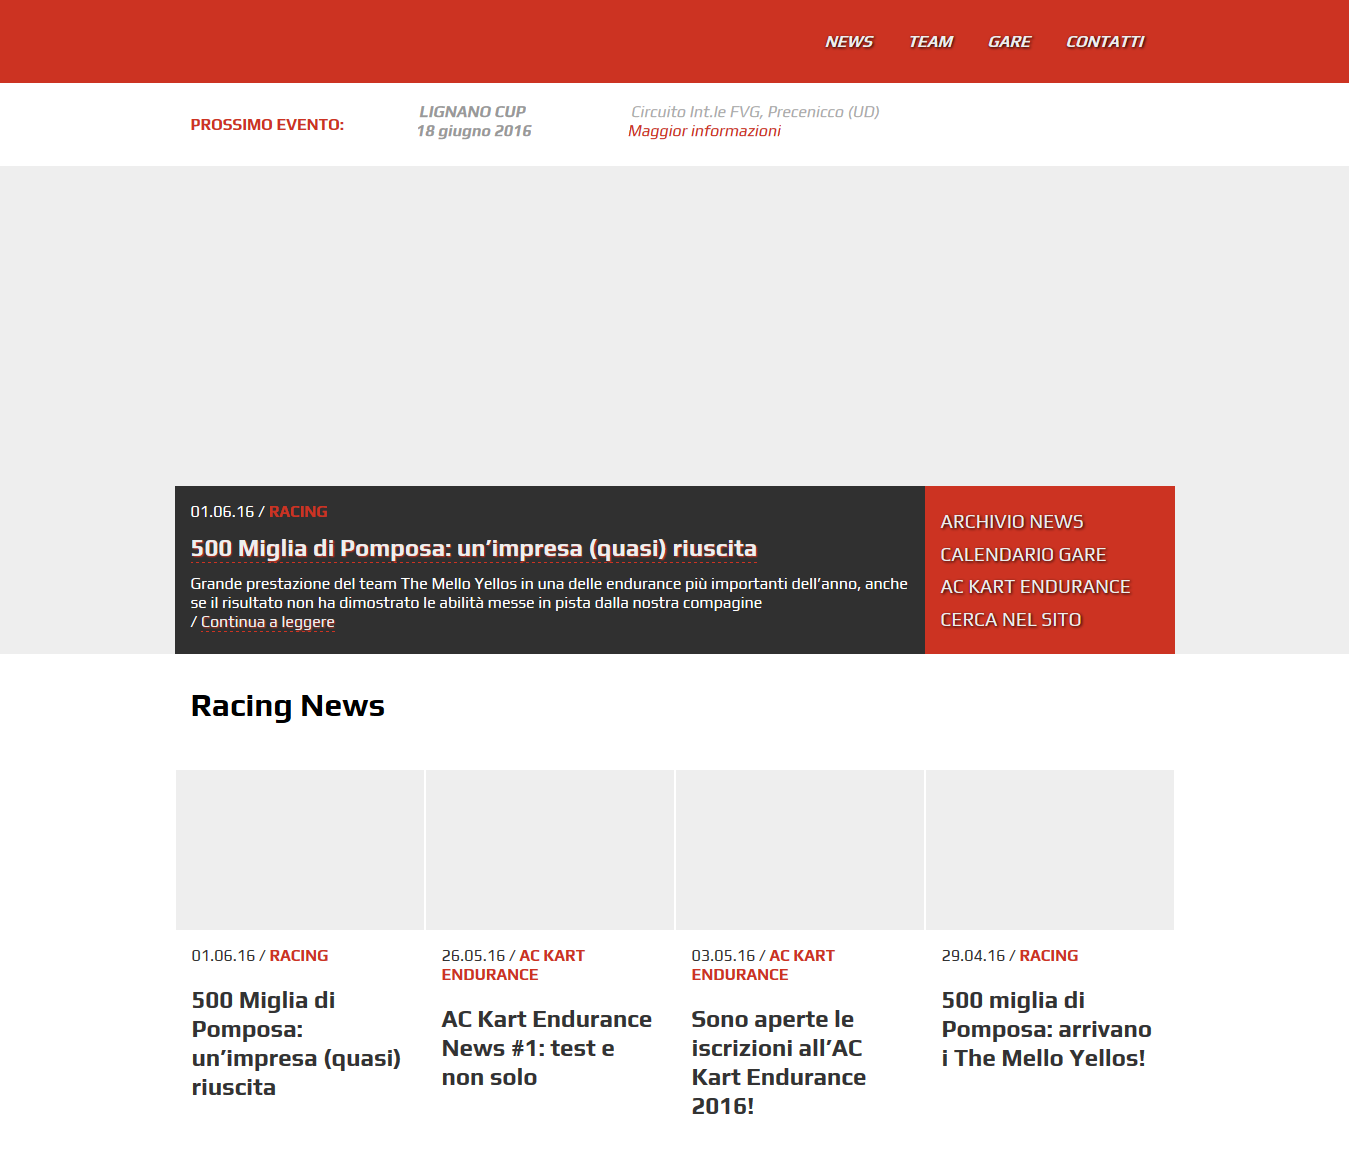
\includegraphics[width=\textwidth]{images/BlankHomepage1}
			\caption{La schermata iniziale della homepage priva di immagini}
			\label{fig:BlankHomepage1}
		\end{figure}
		
		%\begin{figure} [p]
			%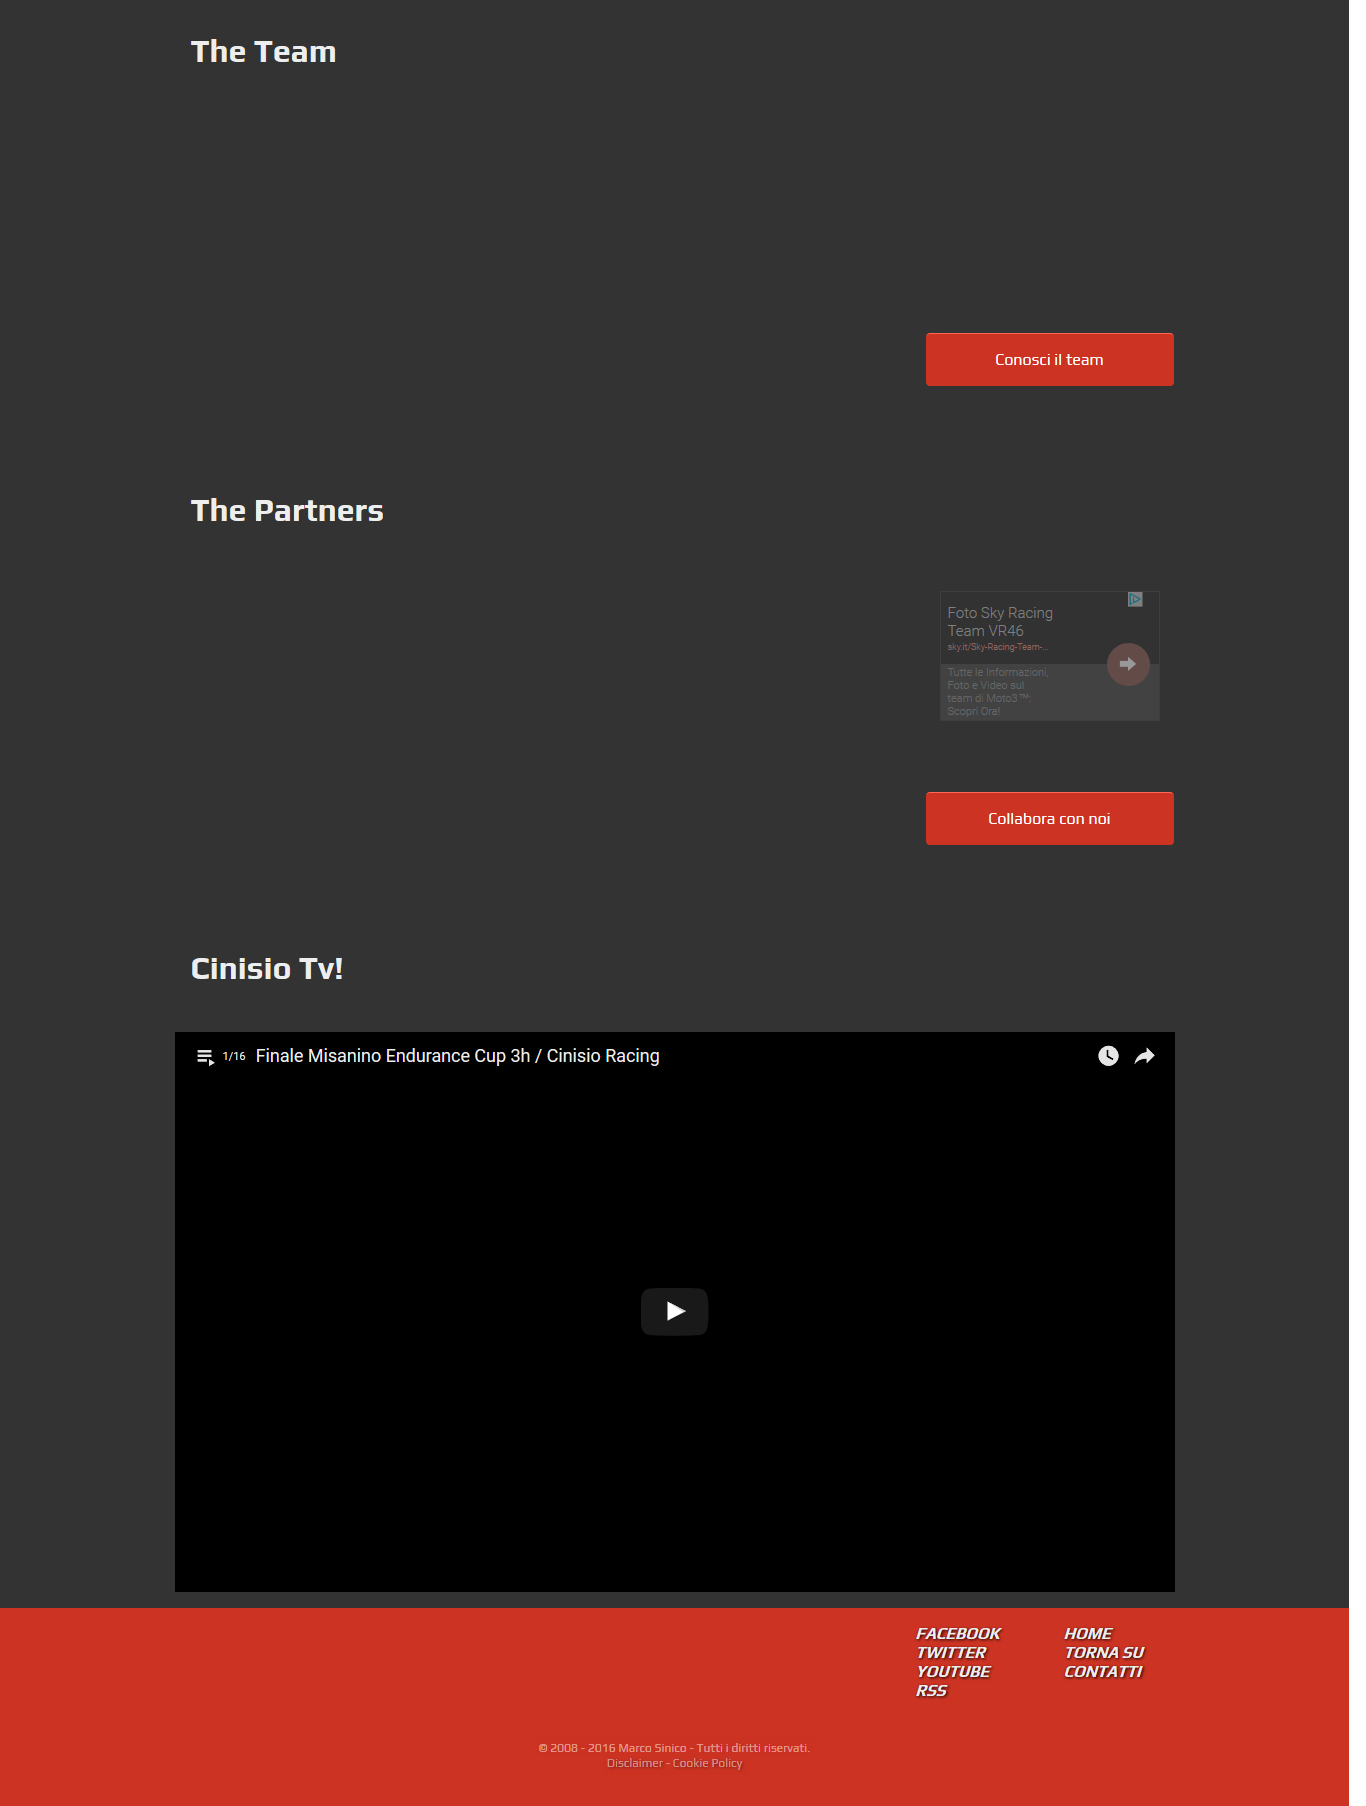
\includegraphics[width=\textwidth]{images/BlankHomepage2}
			%\caption{La homepage priva di immagini (parte 2)}
			%\label{fig:BlankHomepage2}
		%\end{figure}
		
		\newpage
		Da tale figura si può anche intuire quanto lo \textbf{scroll} sia in eccesso solo per dare spazio alle immagini. Il numero di parole all'interno nella pagina infatti è tale da poter essere incluso totalmente nella prima schermata eliminando quasi del tutto l'utilizzo dello scroll.
		
		Inoltre un altro grave riscontro sta nella non ``cliccabilità'' di alcune immagini. Prendendo sempre la homepage come riferimento, si evince che solo le immagini associate ad una new sono cliccabili, tutte le altre no: 
		\begin{itemize}
			\item Immagine a schermo intero delle ultime notizie;
			\item Le immagini del team;
			\item Le immagini che rappresentano gli sponsor.
		\end{itemize}
	
	In conclusione, un'enorme quantità di immagini con più importanza rispetto al testo. La maggioranza di esse non rappresentano link ipertestuali (click a vuoto dell'utente), appesantiscono la dimensione della pagina e sono causa di uno scroll elevato.
	
	\newpage
	\subsection{Cookie policy}
		Un punto a favore va alla gestione dell'avviso dei cookie, il banner di avviso è posizionato in basso alla pagina e non dà in alcun modo fastidio all'utente. Il pulsante per accettare e quindi nascondere l'avviso è bene in vista e facilmente cliccabile. Probabilmente si potrebbe aumentare le sue dimensioni per aumentare l'usabilità nell'impatto iniziale della prima visita.
		 
		\begin{figure} [h]
			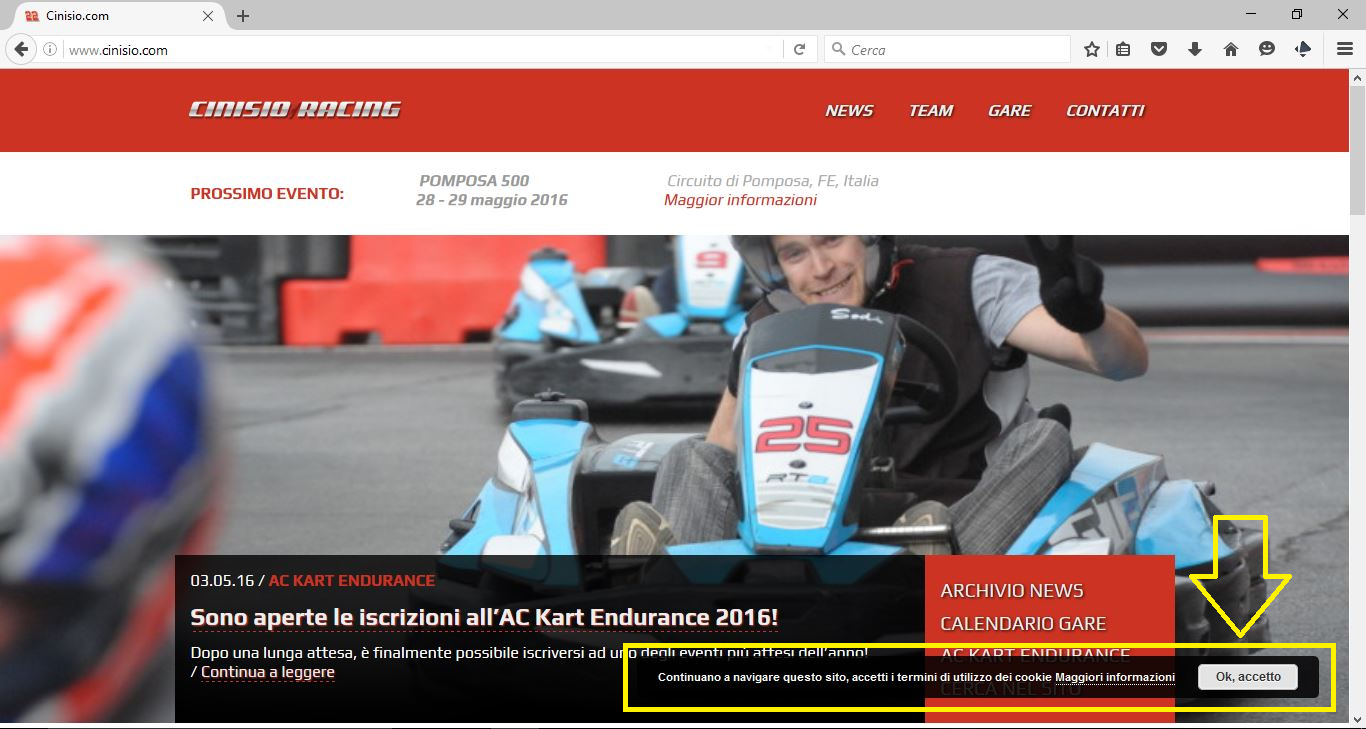
\includegraphics[width=\textwidth]{images/CookiePopUp}
			\caption{Il banner per accettare le policy dei cookie al primo accesso nella homepage}
			\label{fig:CookiePopUp}
		\end{figure}
		 	
	
	\newpage
	\subsection{Breadcrump}
		Il sito presenta un breadcrump solo per le pagine identificate come new o articoli. Il tipo di breadcrump utilizzato è quello ad \textbf{attributi}. Ad ogni new infatti gli viene associato un tag con la tematica che tratta.
		Nonostante questo sia molto utile per comprendere subito l'argomento trattato dall'articolo non soddisfa pienamente i canoni di usabilità. L'utente infatti non sa di essere nella sezione \textbf{news} poiché l'attributo mira solo a distinguere e a classificare le pagine new e non comprendono una visione più larga di tutto il sito.
		
	Risulta quindi necessario un semplice \textbf{location breadcrump} da affiancare agli attributi, purtroppo però questo c'è ma in una posizione errata e quindi invisibile per la maggioranza dell'utenza. Come mostrato in figura \ref{fig:LocationBreadcrump}, il location breadcrump è situato nel titolo della scheda, per cui, oltre ad essere in un luogo raramente consultato dall'utente, l'apertura di più schede comporta la perdita di questo sostituito dal browser con i tre puntini di sospensione (\dots).
		
		\begin{figure} [h]
			
\includegraphics[width=\textwidth]{images/Dettaglio_PathInTheTitleCard}
			\caption{Il location breadcrump nel titolo della scheda}
			\label{fig:LocationBreadcrump}
		\end{figure}
		
		 In conclusione l'utente è privo di un breadcrump robusto su cui agganciarsi in caso di disorientamento. Il breadcrump ad attributi presente risulta insufficiente per la navigazione del sito e il location breadcrump anch'esso presente risulta inutilizzabile data la sua posizione scarsamente consultabile.
		 
	\newpage
	\subsection{Il footer}
		Una nota va fatta anche per la componente in basso ripetuta in tutte le pagine del sito: il footer. Nel sito in esame esso è composto da almeno due schermate di un normale schermo (figure \ref{fig:Footer1} e \ref{fig:Footer2}). Esso è composto dalle seguenti componenti:
		\begin{itemize}
			\item Racing news;
			\item The Team;
			\item The Parteners;
			\item Cinisio TV (solo homepage);
			\item Il footer vero e proprio.
		\end{itemize}
		
		\begin{figure} [h]
			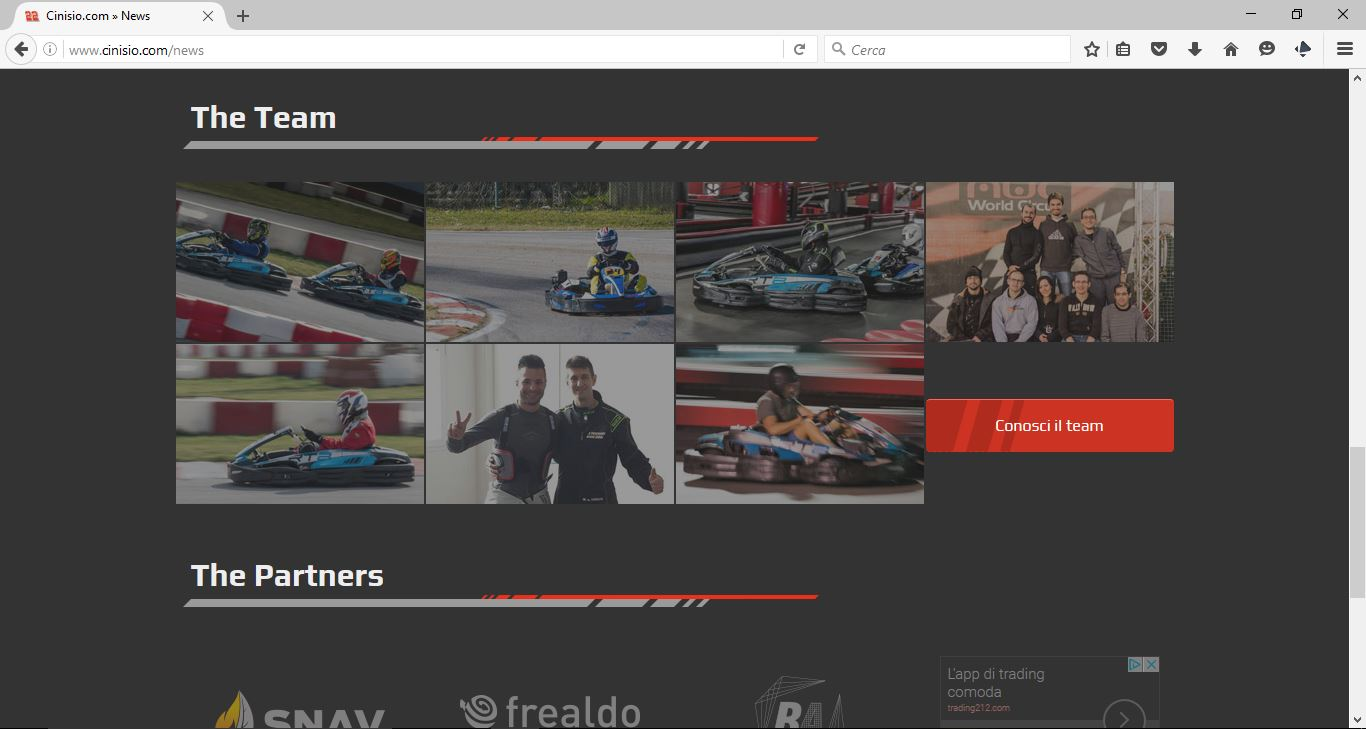
\includegraphics[width=\textwidth]{images/Footer_Part1}
			\caption{Parte 1 che compone il footer}
			\label{fig:Footer1}
		\end{figure}
		
		Per la parte \textbf{Racing new} troviamo due linee con layout a griglia delle ultime news pubblicate. Occupano troppo spazio della pagina (soprattutto negli articoli più lunghi), aumentano inutilmente lo scroll. Una linea di notizie può essere sufficiente anche se essa non dovrebbe essere ripetuta in tutte le pagine, soprattutto quelle degli articoli. Infatti qui è totalmente ridondante poiché esiste già un menu nel lato destro della pagine intitolato \textit{News recenti}
		
		Per quanto riguarda la parte \textbf{The Team} (figura \ref{fig:Footer1}) si può facilmente eliminare o sostituire, le immagini presentate appesantiscono la pagina, generano scroll e non sono cliccabili inoltre il pulsante corrisponde al link del menu se si clicca \textit{TEAM}.
		
		\begin{figure} [h]
			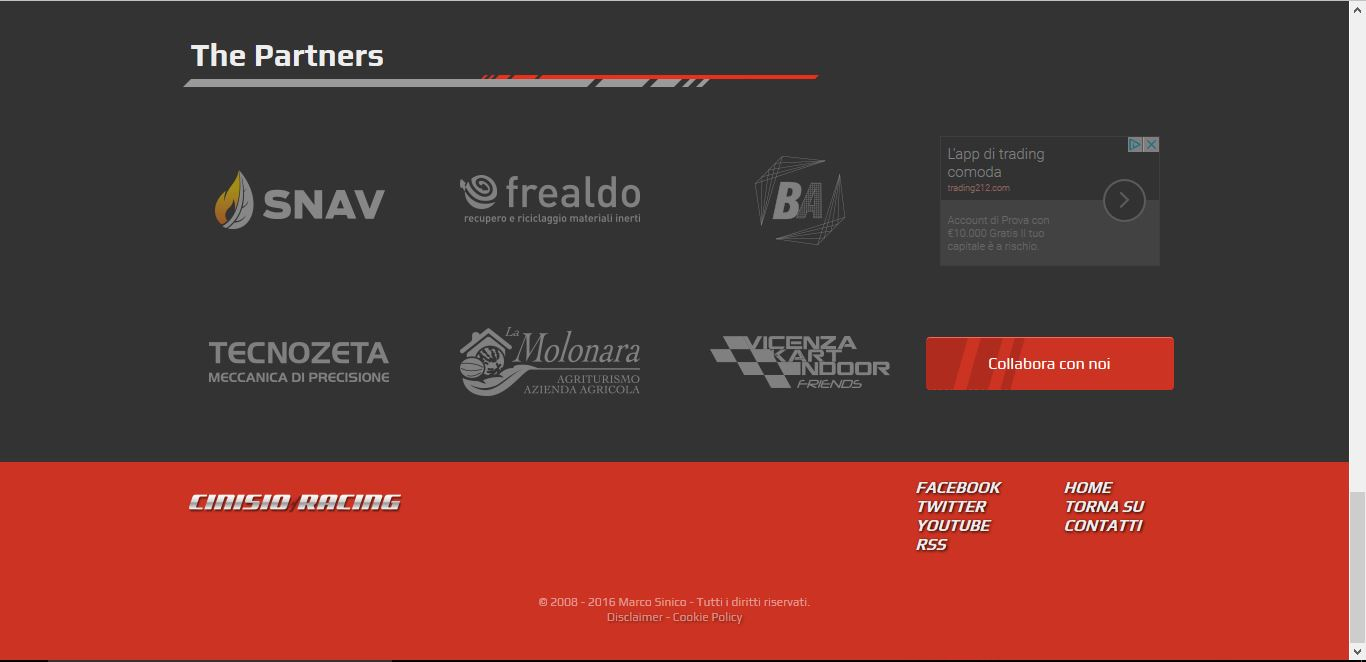
\includegraphics[width=\textwidth]{images/Footer_Part2}
			\caption{Parte 2 che compone il footer}
			\label{fig:Footer2}
		\end{figure}
				
		
		 La parte \textbf{The Partners} (figura \ref{fig:Footer2}) sebbene soffra del problema delle immagini non cliccabili si può accettare come posizionamento anche se con questa posizione nella pagina gli sponsor raramente saranno visti da un utente.	  		

		
		La parte \textbf{Cinisio TV}, disponibile solo nella homepage, invece meriterebbe una pagina dedicata, il player video streaming dal portale YouTube presenta buoni contenuti e funziona solo se richiesto (nessun avvio automatico). Spostarlo dalla homepage favorirebbe la fruizione dei video a tutti quegli utenti che non scrollano fino al footer della homepage e inoltre alleggerirebbe la homepage.
		
		Nell'ultima parte, che è il footer vero e proprio, si presentano i link ai vari social disponibili, stesso errore di prima, un utente non potrà mai usufruire di tali link perché troppo nascosti.
		
		\newpage
		\subsection{Metafore visive}
			Per metafora visiva si intende l'uso di effetti grafici che ingannano l'aspettativa dell'utente. Nel sito sono presenti varie metafore visive. Prima fra tutti quella delle \textbf{immagini} già precedentemente e più volte rimarcata. 
			
			Nella homepage solamente le immagini associate ad un articolo sono cliccabili e conducono l'utente alla pagina di quell'articolo, tutte le altre sono finti link. L'utente in questo caso è ingannato perché le immagini una volta posizionato il cursore su di esse si illuminano con un effetto simile a quello dei link. L'utente in questo caso sarà in condizione di \textit{gambling click} (ossia incerto nell'effetto del click) poiché non sa se tale click causerà uno zoom dell'immagine o l'apertura di una nuova pagina. Non solo, dei due effetti attesi nessuno si manifesterà (metafora visiva) infatti gli effetti del click saranno nulli.
			
			Seconda metafora visiva la troviamo nei \textbf{link}, essi non rispettano lo stile accettato comunemente nel web e lo ridefiniscono in modo complesso. L'utente non ha modo all'interno del sito di capire se un testo è un link e risulta difficile se non impossibile la comprensione di tale stile applicato, poiché cambia di pagina in pagina, infatti solo alcuni dei link già visitati cambiano opportunamente colore. Si sottolinea inoltre che tale errore di usabilità peggiora enormemente la fase di scanning.
			
			La terza e ultima metafora visiva è nelle \textbf{liste}, i classici punti neri affianco ad ogni elemento della lista sono sostituiti con ambigue icone del pulsante conosciuto come \textit{play}, per questo risulta un ottimo inganno per l'utente che si aspetta che tale icona sia cliccabile.
			
		\begin{figure} [h]
			\centering
			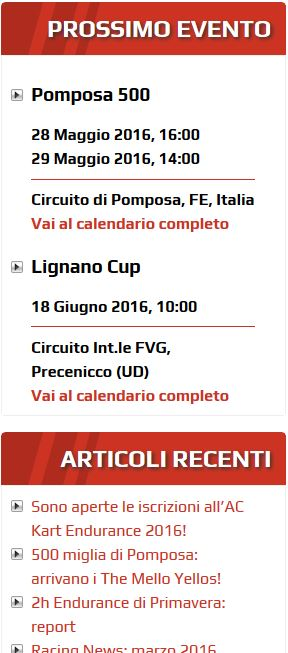
\includegraphics[scale=0.44]{images/MaybeImALink}
			\caption{L'icona ambigua non cliccabile delle liste - in questo caso accompagna dei titoli sopra e dei link cliccabili sotto}
			\label{fig:Footer2}
		\end{figure}
				